%\newpage


\section{Tour of Examples}
\label{sec:tour}

Next, we will walk through a series of examples, in varying levels of complexity. Each example will demonstrate different aspects of serializable vs non-serializable programs.
%
The first examples are relatively basic, while the last examples have higher complexity and are motivated by real-world programs, e.g., BGP routing policy updates.
%
Each thread is spawned any number of times (and at any point in time) by a \textit{request} from the user, marked {\color{ForestGreen}$\blacklozenge_\text{req}$}. The request executes, and eventually return a \textit{response}  {\color{red}$\blacklozenge_\text{resp}$}.
%
For example, in the previous three examples, there is a single request {\color{ForestGreen}$\blacklozenge_\text{main}$} and (up to) two responses {\color{red}$\blacklozenge_0$}, {\color{red}$\blacklozenge_1$}.
% 
We analyze serializability through the lens of such ({\color{ForestGreen}$\blacklozenge_\text{req}$}/{\color{red}$\blacklozenge_\text{resp}$}) pairs. For example, The programs in Listings~\ref{lst:MotivatingExample1Ser}, and~\ref{lst:MotivatingExample3Ser} produce only pairs of the type ({\color{ForestGreen}$\blacklozenge_\text{main}$}/{\color{red}$\blacklozenge_1$}), while the program in Listing~\ref{lst:MotivatingExample2NonSer} can also produce ({\color{ForestGreen}$\blacklozenge_\text{main}$}/{\color{red}$\blacklozenge_0$}). We later formulate this via our network system framework. 
%
We depict global variables with upper-case characters, while local variables (per each request) are depicted with lower-case ones.
%
Unless explicitly stated otherwise, all global and local variables are initialized as 0.
%
The ``\texttt{?}'' symbol depicts a nondeterministic choice between ``0'' and ``1''. All other constructs (\texttt{while}, \texttt{yield}, and \texttt{if}) have their standard interpretation.

\subsection{Example 1}

%\subsubsection{Example 1}

We start with a basic example, describing a single request {\color{ForestGreen}$\blacklozenge_\text{A}$}, a single local variable (``x'') per each request; and a single global variable (FLAG) shared among all in-flight requests. 
%
In Listing~\ref{lst:BasicSer} an in-flight request assigns to x the value of FLAG (hence, initially, [$x:=0$]). Then, the request non-deterministically chooses whether to yield or to flip the value of $x$. Subsequently, FLAG is assigned 1 and the value of x is returned as the response to request {\color{ForestGreen}$\blacklozenge_\text{A}$}. 
%
Note that the presence of the \texttt{else} branch renders the program serializable, as intuitively, 
for any interleaving that modifies \(x\) via the \texttt{if} branch, there exists a corresponding serial execution in which the \texttt{else} branch is taken, yielding an equivalent outcome.
%
However, this changes in  Listing~\ref{lst:BasicNonSer},
%
%
%\begin{wrapfigure}{r}{0.62\textwidth}
%	\vspace{-0.5\intextsep} % tighten top
%	\centering
%	\begin{minipage}[t]{0.25\textwidth}
%		\begin{lstlisting}[caption={Serializable},label={lst:BasicSer},numbers=none]
%request A: 
%    x := FLAG
%
%    if (?):
%        yield
%    else:
%        x := 1 - x
%
%    FLAG := 1
%    return x
%		\end{lstlisting}
%	\end{minipage}\hspace{1.2em}% <-- small gap here
%	\begin{minipage}[t]{0.25\textwidth}
%		\begin{lstlisting}[caption={Not serializable},label={lst:BasicNonSer},numbers=none]
%request A: 
%    x := FLAG 
%
%    if (?): 
%        yield
%    // no else
%
%
%    FLAG := 1 
%    return x
%		\end{lstlisting}
%	\end{minipage}
%	\vspace{-0.9\intextsep} % tighten bottom
%\end{wrapfigure}
%
%
in which there is no ``else'' branch --- an update that makes the program non-serializable.
%
Now, any serial execution will have \textit{at most one} pair of {\color{ForestGreen}$\blacklozenge_\text{A}$}/{\color{red}$\blacklozenge_0$} (this is in fact the first request, returning the original zero-initialized value of FLAG).
%
As the first request also assigns $[FLAG:=1]$ before exiting, any subsequent request in a serial run will assign $[x:=1]$ and hence return only responses of {\color{red}$\blacklozenge_1$}. 
%, and $(i-1)$ pairs of {\color{ForestGreen}$\blacklozenge_\text{A}$}/{\color{red}$\blacklozenge_1$}.
%
%
%
%Any serial execution will match the first request {\color{ForestGreen}$\blacklozenge_\text{A}$} the response {\color{red}$\blacklozenge_0$} (as $[x:=FLAG]$, which is initially 0). 
%
%
%
%
%Differently put, for any serial execution with i requests --- we have exactly one (first) request/response pair {\color{ForestGreen}$\blacklozenge_\text{A}$}/{\color{red}$\blacklozenge_0$}, and $(i-1)$ pairs of {\color{ForestGreen}$\blacklozenge_\text{A}$}/{\color{red}$\blacklozenge_1$}.
%
%\noindent
However, given that the first request can also \textit{yield}, it is possible for another request to concurrently run the program after the first request yields and before it returns. This, in turn, will allow two requests to have $[x=0]$, and hence, for example, we can attain \textit{multiple} {\color{ForestGreen}$\blacklozenge_\text{A}$}/{\color{red}$\blacklozenge_0$} pairs. Thus, Listing~\ref{lst:BasicNonSer} is not serializable.
%\noindent
%\begin{minipage}[t]{0.30\textwidth}
%	\begin{lstlisting}[caption={Serializable},
%		label={lst:BasicSer}]
%request A: 
%    x := FLAG
%
%    if (?):
%        yield
%    else:
%       x := 1 - x
%
%    FLAG := 1
%    return x
%	\end{lstlisting}
%\end{minipage}
%\hfill
%\begin{minipage}[t]{0.30\textwidth}
%	\begin{lstlisting}[caption={Not serializable},
%		label={lst:BasicNonSer}]
%request A: 
%    x := FLAG 
%
%    if (?): 
%        yield
%    // no else
%
%
%    FLAG := 1 
%    return x
%	\end{lstlisting}
%\end{minipage}%


%\todo{original:}

%\vspace{2em}
%example - 2

% Second row
\noindent
\begin{minipage}[t]{0.45\textwidth}
	\begin{lstlisting}[caption={Serializable},
		label={lst:BasicSer},numbers=none]
	request A: 
		x := FLAG
		if (?):
			yield
		else:
			x := 1 - x
		FLAG := 1
		return x
	\end{lstlisting}
\end{minipage}
\hfill
\begin{minipage}[t]{0.45\textwidth}
	\begin{lstlisting}[caption={Not serializable},
	label={lst:BasicNonSer},numbers=none]
			request A: 
			    x := FLAG 
			    if (?): 
			        yield
			    // no else
			
			    FLAG := 1 
			    return x
		\end{lstlisting}
\end{minipage}%

\subsection{Example 2}

%\subsubsection{Example 2}
The following program pairs have a single global variable (X), and two requests --- {\color{ForestGreen}$\blacklozenge_\text{incr}$} which increments X by 1, and {\color{ForestGreen}$\blacklozenge_\text{decr}$} which decrements X by 1. Both programs have loops that guarantee that X will always be between 0 to 3, otherwise the while loop will yield ad infinitum. Both requests return the value of X after updating it.
%
In the first case, Listing~\ref{lst:FredSer} presents a serializable program, due to the absence of any yield between the increment/decrement of X and its return. Equivalently, in each of the requests, the update of X and the returned value can be thought of as \textit{a single atomic execution}.
%
However, in Listing~\ref{lst:FredNonSer}, we add an additional \texttt{yield} (and a local variable ``y''), occurring in each of the requests, between the update of X and its return.
%
This change allows requests of the same type to update X to the same value ---  resulting in outputs such as
$\{{\color{ForestGreen}\blacklozenge_\text{incr}}/{\color{red}\blacklozenge_\text{1}},{\color{ForestGreen}\blacklozenge_\text{incr}}/{\color{red}\blacklozenge_\text{2}},{\color{ForestGreen}\blacklozenge_\text{incr}}/{\color{red}\blacklozenge_\text{3}},{\color{ForestGreen}\blacklozenge_\text{decr}}/{\color{red}\blacklozenge_\text{2}},{\color{ForestGreen}\blacklozenge_\text{decr}}/{\color{red}\blacklozenge_\text{2}}\}$ which cannot be attained in any serial execution.

%
%
%
%  incr/1
%incr/3
%incr/2
%(decr/2)^2
 %

%\vspace{2em}
%\newpage
%example - 3

% Third row
\noindent
\begin{minipage}[t]{0.45\textwidth}
	\begin{lstlisting}[caption={Serializable},
		label={lst:FredSer},numbers=none]
			request incr: 
			    while (X == 3):
			        yield
			        
			        
			    X := X + 1
				  return X		
			
			request decr: 
			    while (X == 0): 
			        yield
			        
			        
			    X := X - 1
				  return X
		\end{lstlisting}
\end{minipage}
\hfill
\begin{minipage}[t]{0.45\textwidth}
	\begin{lstlisting}[caption={Not serializable},
		label={lst:FredNonSer},numbers=none]
			request incr:
			    while (X == 3):
			        yield
			    y := X
			    yield
			    X := y + 1
		      return X		
			
			request decr: 
			    while (X == 0):
			        yield
			    y := X
			    yield
			    X := y - 1
		      return X
		\end{lstlisting}
\end{minipage}
	
\subsection{Example 3}
%\subsubsection{Example 3}	
%\todo{continue}	
%example - 6

The next example (see Listing~\ref{lst:ComplexWhileNonSer}) has a global variable $X$ and a local variable $i$ per each in-flight request. The {\color{ForestGreen}$\blacklozenge_\text{flip}$} request flips $X$ (initialized to 0); the {\color{ForestGreen}$\blacklozenge_\text{main}$} request attempts to decrement $i$ five times.
%
%It is straightforward to observe that the program in Listing~\ref{lst:ComplexWhileSer} is trivially serializable, as there are no yields.
%
Any serial execution does not output any instance of the single response {\color{red}$\blacklozenge_1$}, 
as any serial execution will have a single request in-flight, with $X$ either 0 or 1. Thus, exactly one of the while loops will run indefinitely, prohibiting any {\color{ForestGreen}$\blacklozenge_\text{main}$}/{\color{red}$\blacklozenge_1$} pairs.
%
%Specifically, in any serial execution of requests, the local i variable is either 0 or 1, and hence --- serial execution do no produce any request/response pairs.
%
To show that the program is not serializable, we show that an interleaving \emph{can} result in a non-empty set of outputs. 
%
%However, some interleavings can allow the program to output a response {\color{red}$\blacklozenge_1$}. 
%
Specifically, given at least $i=5$ interleavings of in-flight {\color{ForestGreen}$\blacklozenge_\text{flip}$} requests, it is possible for a {\color{ForestGreen}$\blacklozenge_\text{main}$} request to terminate and bypass all while loops, something that cannot occur in any serial execution.
%
%Here is some text that will flow around the code listing. You can introduce the snippet and then let the text wrap naturally alongside it.

\vspace{1em}  
\begin{wrapfigure}{r}{0.35\textwidth}
	  \vspace{-1em}  % pull the top of the figure up by 1em
	\centering
	\begin{lstlisting}[caption={Not serializable},label={lst:ComplexWhileNonSer},numbers=none]
request flip: 
    X := 1 - X 

request main:
    i := 5
    while (i > 0):
        while (X == 0):
            yield
        while (X == 1):
            yield
        i := i - 1

    return 1        
	\end{lstlisting}
\vspace{-0.5em}  % tighten space at bottom of the listing
\end{wrapfigure}
\vspace{1em}  % space below the wrapfigure; change as needed

%This paragraph will flow to the left of the listing. Continue writing your explanation or narrative here, and the text will neatly wrap around the code block on the right. You can add as much text as you like, and LaTeX will handle the wrapping automatically.

%\bigskip

%If you need to reference the listing elsewhere, use \texttt{\textbackslash ref~\{lst:ComplexWhileNonSer\}} to point to it, e.g., Listing~\ref{lst:ComplexWhileNonSer}.

% Second row
%\noindent
%\begin{minipage}[t]{0.45\textwidth}
%	\begin{lstlisting}[caption={Serializable},
%		label={lst:ComplexWhileSer}]
%		    request flip: 
%		        X := 1 - X 
%		    
%		    request main:
%		        i := 5
%		        while (i > 0):
%		            while (X == 0):
%		                pass
%		            while (X == 1):
%		                pass
%		            i := i - 1
%		        
%		        return 1       
%				\end{lstlisting}
%\end{minipage}%
%\hfill
%\begin{minipage}[t]{0.45\textwidth}
%	\begin{lstlisting}[caption={Not serializable},
%		label={lst:ComplexWhileNonSer}]
%		    request flip: 
%		        X := 1 - X 
%		
%		    request main:
%		        i := 5
%		        while (i > 0):
%		            while (X == 0):
%		                yield
%		            while (X == 1):
%		                yield
%		            i := i - 1
%		
%		        return 1        
%					\end{lstlisting}
%\end{minipage}
	

	
\subsection{Example 4}
%\subsubsection{Example 4: Banking System}


We illustrate a simple banking system inspired by Chandy and Lamport’s distributed snapshot algorithm~\cite{ChLa85}.  The system manages a client’s funds across multiple accounts; we use two accounts, \(A\) and \(B\), but the same pattern extends to any number of accounts.  Each request {\color{ForestGreen}$\blacklozenge_\text{interest}$} applies an arbitrary rate \(t\%\) to every account—we set \(t=100\%\) for simplicity.
%
Each {\color{ForestGreen}$\blacklozenge_{\mathit{transfer}}$} request moves \$50 from \(A\) to \(B\), and each {\color{ForestGreen}$\blacklozenge_{\mathit{interest}}$} request increases every balance by \(t\%\).  Both requests return the combined total \(A + B\).
%
In every serial execution with one {\color{ForestGreen}$\blacklozenge_{\mathit{interest}}$} request, and any number of {\color{ForestGreen}$\blacklozenge_{\mathit{transfer}}$} requests, the total balance satisfies the invariant
$
(A_{\text{after}} + B_{\text{after}})
= (1 + t\%) \,\bigl(A_{\text{before}} + B_{\text{before}}\bigr)
$,
%
%
%\[
%(A_{\text{after}} + B_{\text{after}})
%= (1 + t\%) \,\bigl(A_{\text{before}} + B_{\text{before}}\bigr),
%\]
.  Although the individual balances of \(A\) and \(B\) depend on the chosen serial order, the combined sum always reflects exactly one application of the interest rate.
%
However, non-serial interleavings can violate this invariant.  For instance, if a {\color{ForestGreen}$\blacklozenge_{\mathit{transfer}}$} request deducts \$50 from \(A\) (yielding \([50,50]\)) and then yields, then an {\color{ForestGreen}$\blacklozenge_{\mathit{interest}}$} request may double both balances to \([100,100]\) before the transfer resumes --- resulting in \([100,150]\) and a missing \$50.  By contrast, any correct serial ordering of these two operations yields \(A + B = (100+50)\times2 = 300\), with final states \([150,150]\) or \([100,200]\) depending on which request runs first.
%
%
% original
%The next example emulates a simple banking system, as motivated by Chandy and Lamport's seminal paper on distributed snapshots~\cite{ChLa85}. The system operates on number of bank accounts owned by the same client. For simplicity, we'll choose two bank account denoted by the global variables $A$ and $B$, and initialized to have $100\$$ and $50\$$ respectively. 
%%
%Each {\color{ForestGreen}$\blacklozenge_\text{transfer}$} request allocates $50\$$ from account $A$ to account $B$, and every {\color{ForestGreen}$\blacklozenge_\text{interest}$} request adds $t\%$ interest to each account. For simplicity, and without loss of generality, we chose $t=100\%$, hence doubling the funds in each account, per each such request. We also note that for simplicity we depict two accounts ($A$ and $B$), although this example is valid for any number of accounts.
%%
%Both requests return the final sum of the client funds in both the accounts.  
%%
Listing~\ref{lst:BankSer} has a serial version of this banking system (without \texttt{yield}), and Listing~\ref{lst:BankNonSer} includes yields between the adjustment of accounts $A$ and $B$ (we note that this also represents real-world systems in which the account can be sharded and partitioned across different nodes).
%


\noindent
\begin{minipage}[t]{0.45\textwidth}
	\begin{lstlisting}[caption={Serializable},
		label={lst:BankSer},numbers=none]
	    A := 100, B := 50
	    
	    request transfer: 
	        // transfer 50$
	        A := A - 50
	        // no yield
	        B := B + 50
	        return A + B
				
	    request interest: 
	        // add a 100% interest
	        A := A + A
	        // no yield
	        B := B + B
	        return A + B      
			\end{lstlisting}
\end{minipage}
\hfill
\begin{minipage}[t]{0.45\textwidth}
	\begin{lstlisting}[caption={Not serializable},
		label={lst:BankNonSer},numbers=none]
	    A := 100, B := 50
			
	    request transfer: 
	        // transfer 50$
	        A := A - 50
	        yield
	        B := B + 50
	        return A + B
	
	    request interest: 
	        // add a 100% interest
	        A := A + A
	        yield
	        B := B + B
	        return A + B
      		\end{lstlisting}
\end{minipage}
	

%Interestingly, in this setting, serializability also corresponds to correctness invariants pertaining to the program. Specifically, in every serializable execution, it holds that for $A_{\textit{before}},B_{\textit{before}}$ marking the funds before running a single {\color{ForestGreen}$\blacklozenge_\text{interest}$} request, and any number of {\color{ForestGreen}$\blacklozenge_\text{transfer}$} requests (and $A_{\textit{after}},B_{\textit{after}}$ marking the corresponding state after those requests), then:
%\[
%\bigl(A_{\mathit{after}} + B_{\mathit{after}}\bigr)
%= (1 + t\%)\,\bigl(A_{\mathit{before}} + B_{\mathit{before}}\bigr).
%\]
%
%This invariant always holds for any such serial execution, while having the specific division \textit{between} accounts $A$ and $B$ depending on the actual order of the serial execution.
%%
%However, this correctness invariant does not hold for non serializable executions. For example, in a setting in which there is a single {\color{ForestGreen}$\blacklozenge_\text{transfer}$} request, which deduces $50\%$ from account $A$, and then yields (resulting to a temporary state in which $[A=50\$,B=50\$]$); subsequently followed by an  {\color{ForestGreen}$\blacklozenge_\text{interest}$} request which runs until completion, in which case  $[A=100\$,B=100\$]$, and then, the remainder of the yielded {\color{ForestGreen}$\blacklozenge_\text{transfer}$} request is executed, resulting finally to $[A=100\$, B=150\$]$.  This result in $50\$$ ``missing'' from our system, due to this non serializable behavior.
%%
%As mentioned, a serial execution of a these two request will always result to 
%$A+B=2\cdot (100\$+50\$)=300\$$, with either a final state of $[A=150\$, B=150\$]$ or $[A=100\$, B=200\$]$, depending on the scheduled serializable order.




%\newpage
\subsection{Example 5}

The following example is motivated by~\cite{NaGhSa24} and demonstrates how reasoning about serializability corresponds to correctness in routing policies in software‐defined networking (SDN). In SDN, switches not only forward packets but can also be programmed in domain‐specific languages (e.g., P4). At runtime, a centralized controller node can adjust the global network control policy. The controller can also periodically send control packets to each switch, causing it to adjust its routing policy as dictated by the updates.
%
An instance of a simple network with two competing policies is shown in Fig.~\ref{fig:BgpRoutingPolicies}. This network consists of four nodes (numbered 0 through 3), with the two middle nodes --- node 1 (labeled WEST) and node 2 (labeled EAST), serving as ingress points from where traffic nondeterministically enters the network. The controller selects one of two policies: a \textcolor{NavyBlue}{blue} policy, which routes traffic from West to East, or an \textcolor{darkorange}{orange} policy, which routes it in the opposite direction.
%
%
%// [WEST, switch 1] ---> [EAST, switch 2] ---> [out, switch 3] 
%else:
%B := 0 // red/orange policy
%// [out, switch 0] <--- [WEST, switch 1] <--- [EAST, switch 2] 
%
\begin{wrapfigure}{r}{0.45\textwidth}  % “r” = wrap on the right, width = 45% of line
	\centering
	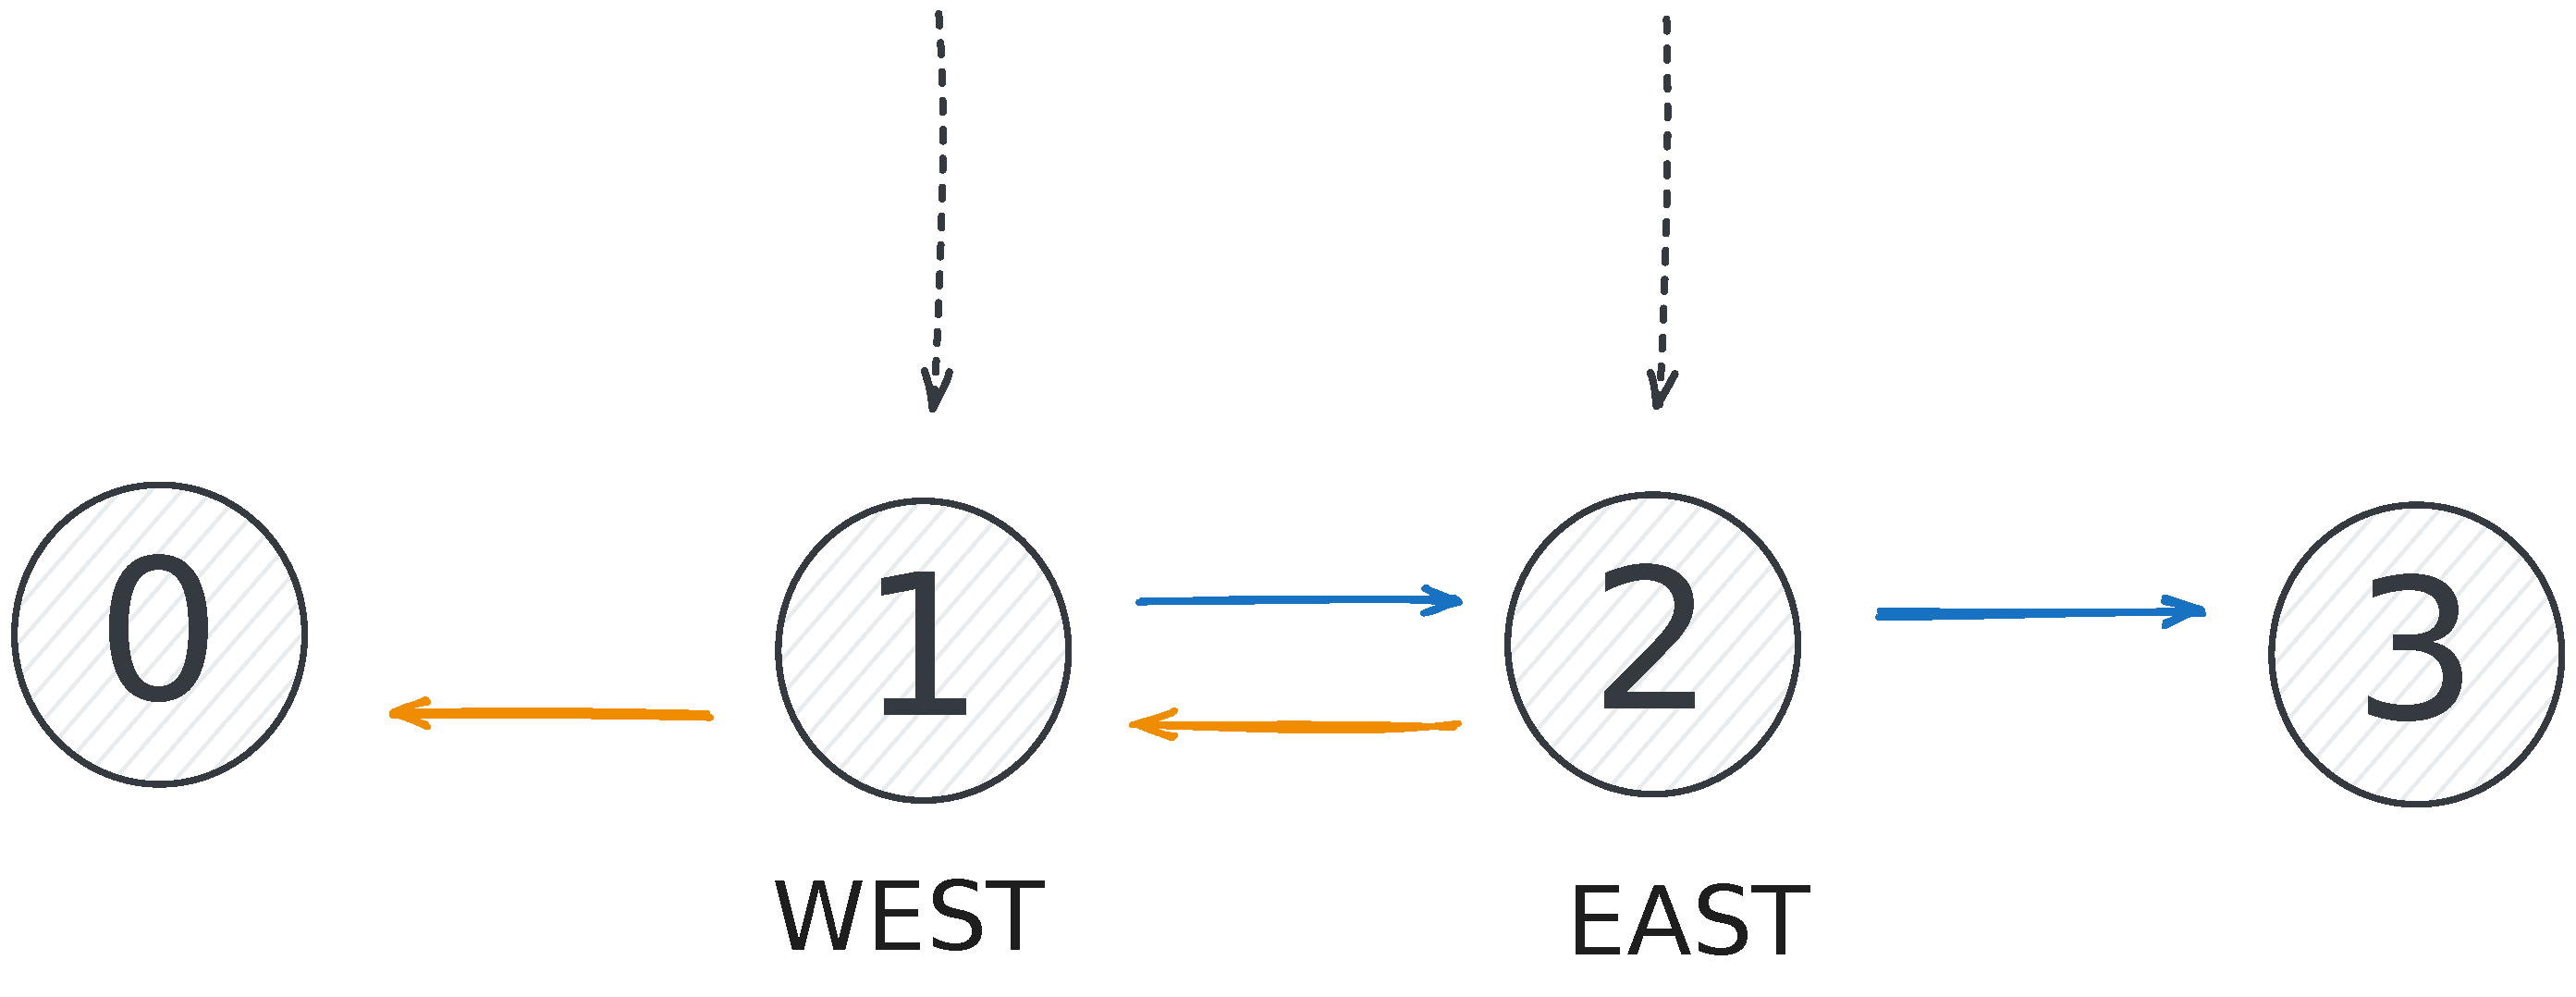
\includegraphics[
	width=\linewidth,
	trim=10 15 15 5,   % {left bottom right top} — tweak as needed
	clip
	]{plots/east_west_routing_updated_colors.pdf}
	\caption{Two routing policies.}
	\label{fig:BgpRoutingPolicies}
\end{wrapfigure}
%
%\begin{figure}[H]
%	\centering
%	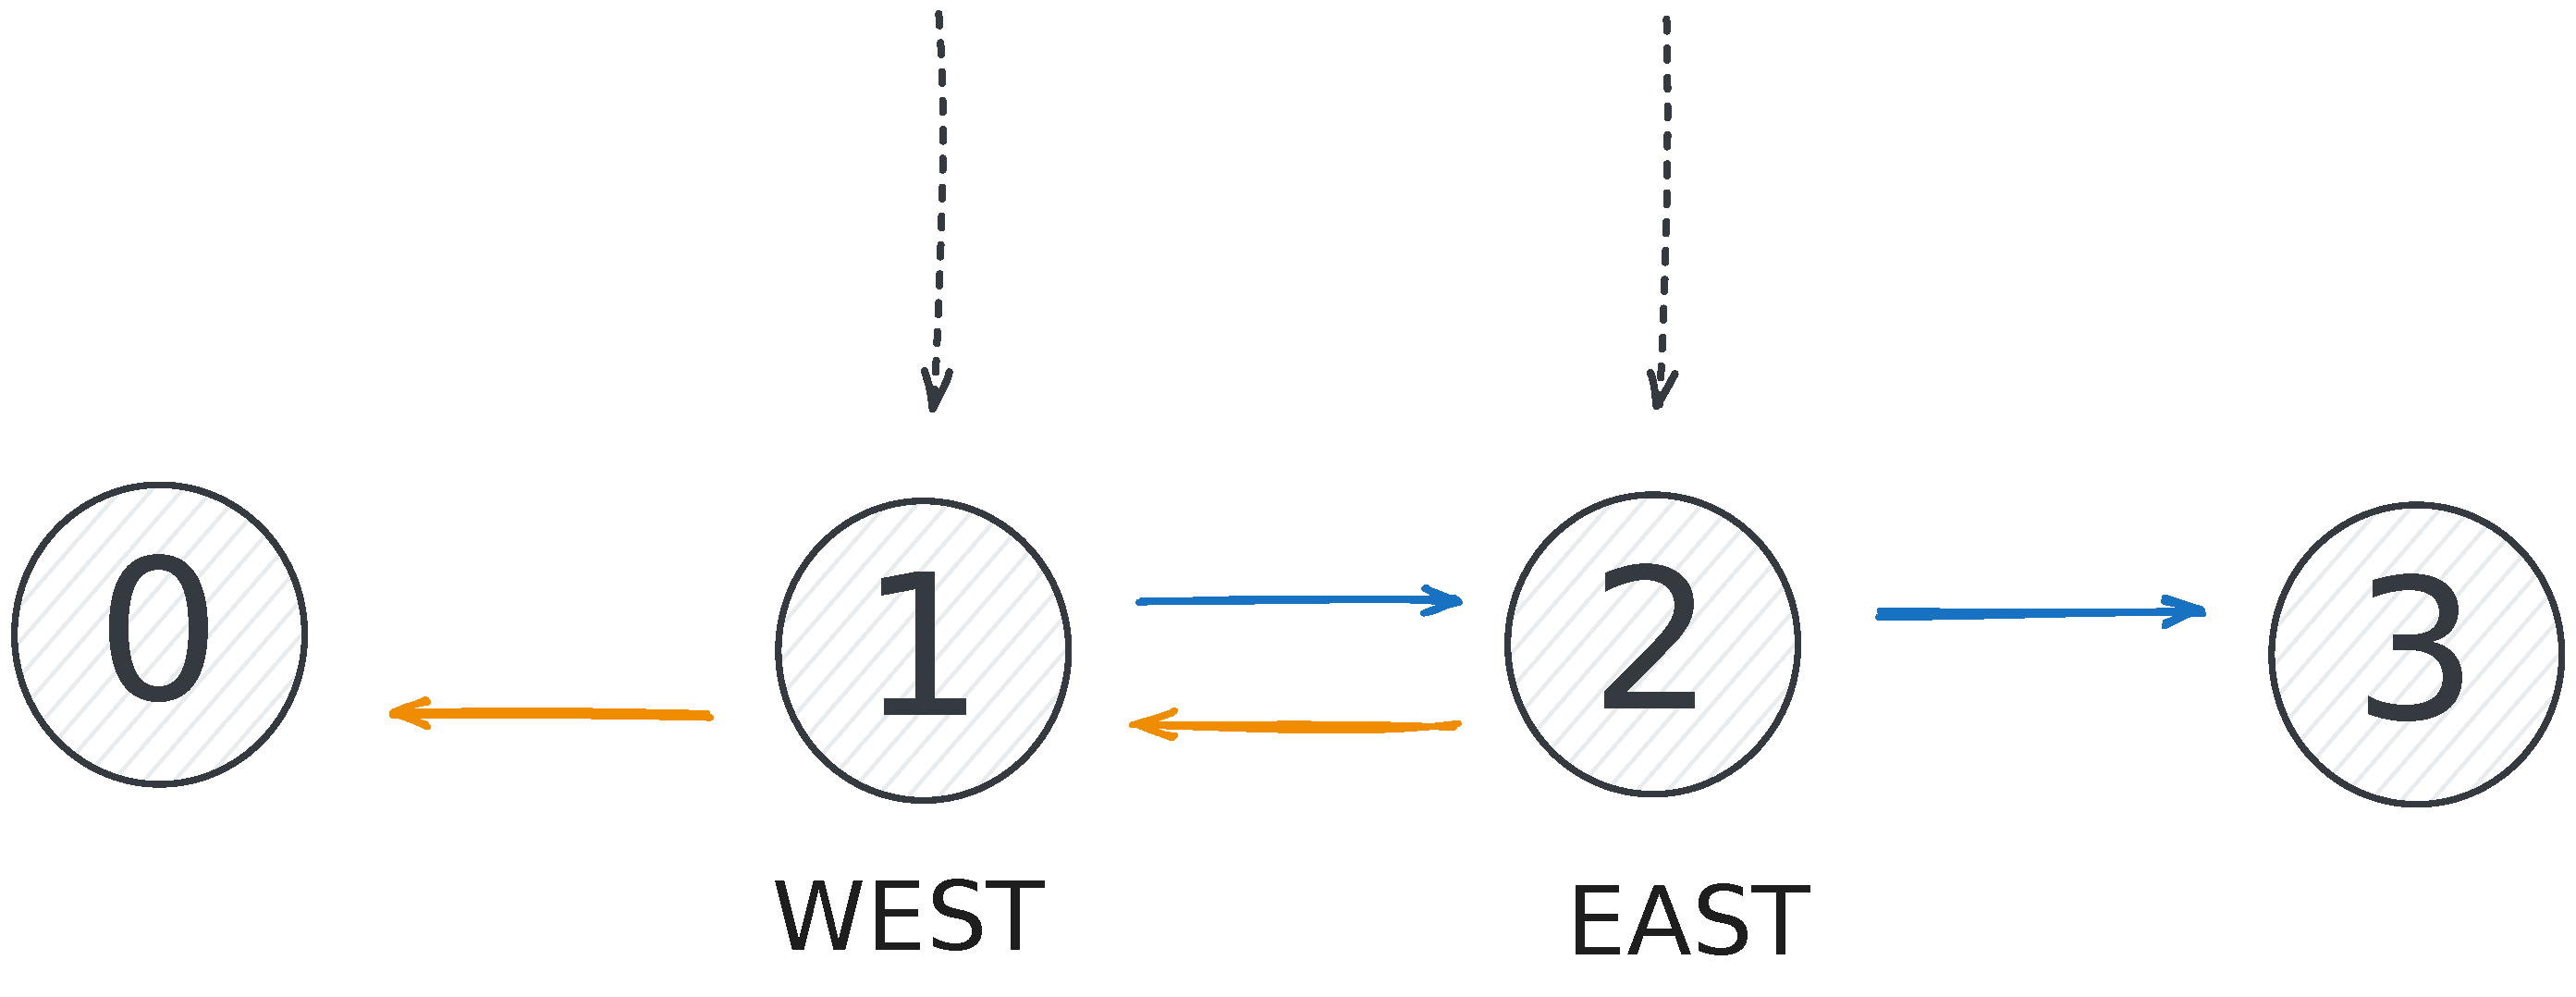
\includegraphics[width=0.5\linewidth]{plots/east_west_routing_updated_colors.pdf}
%	\caption{Routing policy in example 5.}
%	\label{fig:BgpRoutingPolicies}
%\end{figure}
%
This SDN-controlled routing policy is realized in the pseudo-code in Listing~\ref{lst:BgpNonSerializable}.
%
The program includes a single global variable $B$, indicating whether the current routing policy is \textcolor{NavyBlue}{blue} ($[B=1]$) or \textcolor{darkorange}{orange} ($[B=0]$).
%
The program has three types of requests:
%\begin{itemize}
%	
%	\item
	(i)
	{\color{ForestGreen}$\blacklozenge_\text{policy update}$}:
%	\textit{policy update}:
 represents a controller  update, which nondeterministically decides whether to update the policy (i.e., flip the value of  variable $B$) or not;
%	
%		\item
(ii)
	{\color{ForestGreen}$\blacklozenge_\text{route\_west}$}:
	 a request representing a packet entering the network from the \textit{WEST} node; and 
%	
%		\item
(iii)
{\color{ForestGreen}$\blacklozenge_\text{route\_east}$}: a request representing a packet entering the network from the EAST node.
	%
%\end{itemize}
%
%Each of the routing requests represents a single packet entering the network. The request includes a local \textit{current} variable representing the index of the current node visited. This variable is initialized as the ingress node value, and updated to emulate the chosen routing path. There is also a \textit{visited\_east} variable (or a \textit{visited\_west} variable, depending on the request in question).
%%
%The return value of the {\color{ForestGreen}$\blacklozenge_\text{route\_from\_west}$} requests is the sum \textit{(current+current+visited\_east)}. This is an identifier encoding all possible \textit{(current\_switch, visited\_east)} pairs.
%%
%The program is not serializable, as witnessed by an interleaving that can give rise to final return value of \textit{(current+current+visited\_east)=1} (due to \textit{current=0} and \textit{visited\_east=1}). This represents a routing cycle in the network, which is possible only when updated the routing policy after a request has already been routed based on the previous policy.
%Legal, acyclic routes of this request have either a return value of 0 (in the case of [\textit{current=0}, \textit{visited\_east=0}]) or 7 (in the case of [\textit{current=3}, \textit{visited\_east=1}]).
%Potential routing cycles can also be observed via non serializable executions also for the  {\color{ForestGreen}$\blacklozenge_\text{route\_from\_east}$} requests.


\begin{center}
\begin{minipage}[!htbp]{0.85\textwidth}
	\begin{lstlisting}[caption={BGP routing (not serializable)},label={lst:BgpNonSerializable},numbers=none]
 request policy_update:
     if (?): // nondeterministically 1 or 0
         B := 1  // blue policy 
     else:
         B := 0 // orange policy
		
 request route_west:
     current := 1 // initial node
     while (current == 2) or (current == 3): // still routing        
         if (current == 1): // west (switch 1)
             if (B == 1): // blue policy
                 current := 2
             else: // orange policy
                 current := 0
         if (current == 2): // east (switch 2)
             visited_east := 1
             if (B == 1): // blue policy
                 current := 3
             else: // orange policy
                 current := 1
         yield
     return current + current + visited_east
     
 request route_east: ... // dual case      
		\end{lstlisting}
\end{minipage}
\end{center}


Each of the routing requests represents a single packet entering the network. The request includes a local \texttt{current} variable representing the index of the current node visited. This variable is initialized as the ingress node value, and updated to emulate the chosen routing path. There is also a \texttt{visited\_east} variable (or a \texttt{visited\_west} variable, depending on the request in question).
%
The return value of the {\color{ForestGreen}$\blacklozenge_\text{route\_west}$} requests is the sum \texttt{(current+current+visited\_east)}, an identifier encoding all possible \texttt{(current\_switch, visited\_east)} pairs.
%
The program is not serializable, as witnessed by an interleaving that can give rise to a final return value of \texttt{(current+current+visited\_east)=1} (due to \texttt{current=0} and \texttt{visited\_east=1}). This represents a routing cycle in the network, which is possible only when there is an interleaving between a control packet ({\color{ForestGreen}$\blacklozenge_\text{policy\_update}$}) and a routing packet ({\color{ForestGreen}$\blacklozenge_\text{route\_west}$}). Specifically, this occurs when a request has already been spawned based on the previous policy, subsequently yields, and eventually returns after the policy was flipped based on another control packet --- hence resulting in a routing cycle.
%
More formally, this is conveyed by return values that represent these cycles and are attained only via non-serializable executions. For example, legal, acyclic routes of this request have either a return value of 0 (in the case of [\texttt{current=0}, \texttt{visited\_east=0}]) or 7 (in the case of [\texttt{current=3}, \texttt{visited\_east=1}]).
Dually, routing cycles also occur in the case of {\color{ForestGreen}$\blacklozenge_\text{route\_east}$} interleavings.


\subsection{Example 6}
We include an additional network‐monitoring example under \textit{snapshot isolation} in Appendix~\ref{appendix:snapshotIsolationExample}. Snapshot isolation is supported by production databases such as \texttt{PostgreSQL}~\cite{postgresql-transaction-iso} and \texttt{CockroachDB}~\cite{cockroachdb-si-docs}, and has been linked to real‐world anomalies (e.g., duplicate‐key errors in the latter~\cite{cockroach-issue-14099}).

%We add an additional example for network monitoring and \textit{snapshot isolation} in Appendix~\ref{appendix:snapshotIsolationExample}. Snapshot isolation is a consistency model used in production systems such as \texttt{PostgreSQL}~\cite{postgresql-transaction-iso} and \texttt{CockroachDB}~\cite{cockroachdb-si-docs}, and has been implicated in real-world bugs (e.g.,see the report on duplicate key errors ins \texttt{CockroachDB}~\cite{cockroach-issue-14099}).


%We add an additional example for network monitoring and \textit{snapshot isolation} in Appendix~\ref{appendix:snapshotIsolationExample}.%, and its relation to serializability.
%\guy{suddenly I'm not so sure about this example. It is indeed sound but maybe a bit silly?}



